%latex model.tex
%bibtex model
%latex model.tex
%latex model.tex
%dvipdfm model.dvi

%se poate lucra si online (de ex www.overleaf.com)


\documentclass[runningheads,a4paper,11pt]{report}

\usepackage{algorithmic}
\usepackage{algorithm} 
\usepackage{array}
\usepackage{amsmath}
\usepackage{amsfonts}
\usepackage{amssymb}
\usepackage{amsthm}
\usepackage{caption}
\usepackage{comment} 
\usepackage{epsfig} 
\usepackage{fancyhdr}
\usepackage{geometry} 
\usepackage{graphicx}
\usepackage[colorlinks]{hyperref} 
\usepackage[latin1]{inputenc}
\usepackage{multicol}
\usepackage{multirow} 
\usepackage{rotating}
\usepackage{setspace}
\usepackage{subfigure}
\usepackage{url}
\usepackage{verbatim}
\usepackage{xcolor}

\geometry{a4paper,top=3cm,left=2cm,right=2cm,bottom=3cm}

\pagestyle{fancy}
\fancyhf{}
\fancyhead[LE,RO]{Emotion recognition}
\fancyhead[RE,LO]{Team 3}
\fancyfoot[RE,LO]{ITSG 2019-2020}
\fancyfoot[LE,RO]{\thepage}

\renewcommand{\headrulewidth}{2pt}
\renewcommand{\footrulewidth}{1pt}
\renewcommand{\headrule}{\hbox to\headwidth{%
  \color{lime}\leaders\hrule height \headrulewidth\hfill}}
\renewcommand{\footrule}{\hbox to\headwidth{%
  \color{lime}\leaders\hrule height \footrulewidth\hfill}}

\hypersetup{
pdftitle={artTitle},
pdfauthor={name},
pdfkeywords={pdf, latex, tex, ps2pdf, dvipdfm, pdflatex},
bookmarksnumbered,
pdfstartview={FitH},
urlcolor=cyan,
colorlinks=true,
linkcolor=red,
citecolor=green,
}
% \pagestyle{plain}

\setcounter{secnumdepth}{3}
\setcounter{tocdepth}{3}

\linespread{1}

% \pagestyle{myheadings}

\makeindex


\begin{document}

\begin{titlepage}
\sloppy
\begin{center}
BABE\c S BOLYAI UNIVERSITY, CLUJ NAPOCA, ROM\^ ANIA

FACULTY OF MATHEMATICS AND COMPUTER SCIENCE

\vspace{6cm}

\Huge \textbf{Kids Emotion Recognition}

\vspace{1cm}

\normalsize -- ITSG report --

\end{center}


\vspace{5cm}

\begin{flushright}
\Large{\textbf{Team members}}\\
Almasan-Tigau Alexandra \\
Gorgos Andreea \\
Corman Robert-Marian \\
\end{flushright}

\vspace{4cm}
l
\begin{center}
2019
\end{center}

\end{titlepage}

\pagenumbering{gobble}

\tableofcontents

\newpage

\newpage

\setstretch{1.5}



\newpage

\pagenumbering{arabic}


 

\chapter{Neural Networks}
\label{chapter:neuralnetworks}
\section{Introduction of neural networks}
\label{section:introduction_neural_networks}
\textbf{Neural Networks} are a set of algorithms, modeled mainly after the human brain, that are designed to identify and recognize different types of patterns. The patterns that the algorithms recognize are numerical, contained in vectors, into which all real-world data, be it images, sound, text or time series, must be translated.
Neural networks can be seen as a clustering and classification layer on top of the data that needs to be stored and managed. They help to group unlabeled data according to similarities between the example inputs. 
All classification tasks depend upon labeled datasets. In other words, humans must transfer their existing knowledge to the dataset so a neural network to learn the correlation between labels and data. This is known as supervised learning and brings value for:
\begin{itemize}
	\item Detect faces, identify people in images, \textbf{recognize facial expressions}
	\item Recognize gestures in video
	\item Identify objects in images
\end{itemize} and many others.\cite{skymindneural}
\section{Neural Networks Elements}
\label{section:neural_networks_elements}
Neural networks are the networks compose of several \textbf{layers}. 
The layers are made of \textbf{nodes}. A node is a place where computation happens, meaning that it combines input from the data with a set of coefficients, or weights, that either amplify of dampen that input. These input-weight products are summed and then the sum is passed to an \textbf{activation function} (of a node) to determine if the signal should progress further through the network in order to affect the final outcome. If this happens and the signals passes, then the neuron's status is active.\cite{skymindneural,machinelearning}
\chapter{Algorithm: Convolutional Neural Networks}
\label{chapter:cnn}

\section{What?}
\label{section:what}
A \textbf{Convolutional Neural Network (CNN)} is a type of artificial neural network used in image recognition and processing that is specifically designed to process data based on its pixels. A CNN is a Deep Learning algorithm which can take in an input image, assign importance (weights) to various aspects in the image and be able to differentiate one from the other. Traditional neural networks are not ideal for image processing and must be fed images in reduced-resolution pieces. CNN have their "neurons" (nodes) arranged more like those of the frontal lobe, the area responsible for processing visual stimuli in humans.\cite{searchwhat}
\section{Architecture}
\label{section:architecture}
A Convolutional Neural Network consists of a number of convolutional layers optionally followed by fully connected layers.The input of a layer is a $\textbf{\textit{m}} \times \textbf{\textit{m}} \times \textbf{\textit{r}}$ image, where m is the height and width of the image and r is the number of channels (for example, in case of an RGB image, \textbf{\textit{r} = 3)}. The convolutional layer will have \textbf{\textit{k}} filter/kernels of size $\textbf{\textit{n}} \times \textbf{\textit{n}} \times \textbf{\textit{q}}$ where n is smaller than the dimension of the image and q can either be the same as the number of channels r or smaller. Out of these data there can be produces \textbf{k} feature maps of size \textbf{m-n+1}.\cite{stanford}.
\section{How?}
\label{section:how}
In the context of a convolutional neural network, a convolution is a linear operation that involves multiplication of a set of inputs with a set of weights, just as described in the previous chapter of Neural Networks. Given that the technique was designed for two-dimensional input, the multiplication is performed between an array of input data and a two-dimensional array if weights called filter.
The results of previous multiplications are then summed and in the end a single value is returned, that is why the operation is often called \textbf{scalar product} (between inputs and weights). Usually, the filter is smaller than the input and this detail allows the same set of weights to be multiplied by the input array multiple times at different points of the input. As the filter is applied multiple times to the input array, the result is a two-dimensional array of output values that represents a filtering of the input. As such, the two-dimensional output array from this operation is called a \textbf{feature-map}.
So convolutional networks perform a sort of search among the provided image and try to find the previously generated feature-map among the initial image. Each time a match is found, it is mapped onto a feature space particular to that visual element. In that space, the location of each match is recorded. 
\cite{machinelearning}

Our aim was to find an algorithm that has already attained good results in detecting adult facial emotions and train it to recognize children facial emotions while maintaining the highest level of results' accuracy.  \newline

\textbf{Adults' emotion recognition results}e

The ratio used was: 80-10-10 for training-validation-test sets.

The best result obtained:  71.161\% accuracy \cite{adultdata}\newline

\textbf{Children emotion recognition results}

The ratio used was: 80-10-10 for training-validation-test sets.

The best result obtained:  65.5335\% accuracy \newline


\section{Methodology}
\label{section:methodology}

\begin{itemize}
	\item What are criteria you are using to evaluate your method?
  \paragraph{}
  Accuracy. The accuracy of a model is usually determined after the model parameters are learned and fixed and no learning is taking place.
	\item What specific hypotheses does your experiment test? Describe the experimental methodology that you used.
  \paragraph{}
  It's testing how well algorithm that does classification for emotions on people faces.
	\item What are the dependent and independent variables?
  \begin{itemize}
    \item Learning Rate: 0.001
    \item Adam optimizer
    \item categorical\_crossentropy loss
  \end{itemize}

	\item What is the training/test data that was used, and why is it realistic or interesting? Exactly what performance data did you collect and how are you presenting and analyzing it? Comparisons to competing methods that address the same problem are particularly useful.
  \paragraph{}{FER 2013 Dataset}

  \begin{itemize}
    \item Does not contain kids images
    \item Traning acc (90\% from dataset): 98.64\% - Test acc (10\% from dataset): 67.24\% (a bit of overfitting)
  \end{itemize}

  \paragraph{CAFFE Dataset}

  \begin{itemize}
    \item Data are unbalanced
    \item Labeling seems to be wrong (sad seems neutral or others)
    \item Has open mouth faces (e.g. for sad, neutral)
    \item Traning acc (90\% from dataset): 89.94\% - Test acc (10\% from dataset): 67.59\% (a bit of overfitting) - also removing the open mouth images
    \item Contains only kids images
  \end{itemize}

\end{itemize}

\section{Data}
\label{section:data}

\paragraph{FER}

The data consists of 48x48 pixel grayscale images of faces. The faces have been automatically registered so that the face is more or less centered and occupies about the same amount of space in each image. The task is to categorize each face based on the emotion shown in the facial expression in to one of seven categories (0=Angry, 1=Disgust, 2=Fear, 3=Happy, 4=Sad, 5=Surprise, 6=Neutral).

train.csv contains two columns, "emotion" and "pixels". The "emotion" column contains a numeric code ranging from 0 to 6, inclusive, for the emotion that is present in the image. The "pixels" column contains a string surrounded in quotes for each image. The contents of this string a space-separated pixel values in row major order. test.csv contains only the "pixels" column and your task is to predict the emotion column.

\paragraph{CAFFE}
To train the algorithm for facial recognition we have used the data set provided by the Child Study Center at Rutgers University, New Jersey.
The Child Affective Facial Expressions Set (CAFE)\cite{cafe} represents the first large representative database of children posing using many facial expressions.
% \begin{figure}[htbp]
% 	\centerline{\includegraphics{child emotions.png}}
% 	\caption{Example of the child images included in the CAFE data set.}
% 	\label{swarmsize}
% \end{figure}
This data set consists of approximately 1200 photographs of over 100 children racially and ethnically diverse (90 female models and 64 male models: 27 African American, 16 Asian, 77 Caucasian/European American, 23 Latino, and 11 South Asian)with ages between 2 and 8 years old, that are posing 7 different facial expressions:  happy, angry, sad, fearful, surprise, neutral and disgust.


The institute focuses their research on the cognitive, emotional and perceptual development of infants and children. To gather all these visual records, the institute is inviting all families having a child with age between 3 and 8 years, to take part in the study by bringing their child to a session of 30-45 minutes of computer interactive games or of a stimulating reading session. The children are verbally invited to pose each of the emotion with their mouth open and with their mouth closed.

\section{Results}
\label{section:results}

% \begin{figure}[htbp]
% 	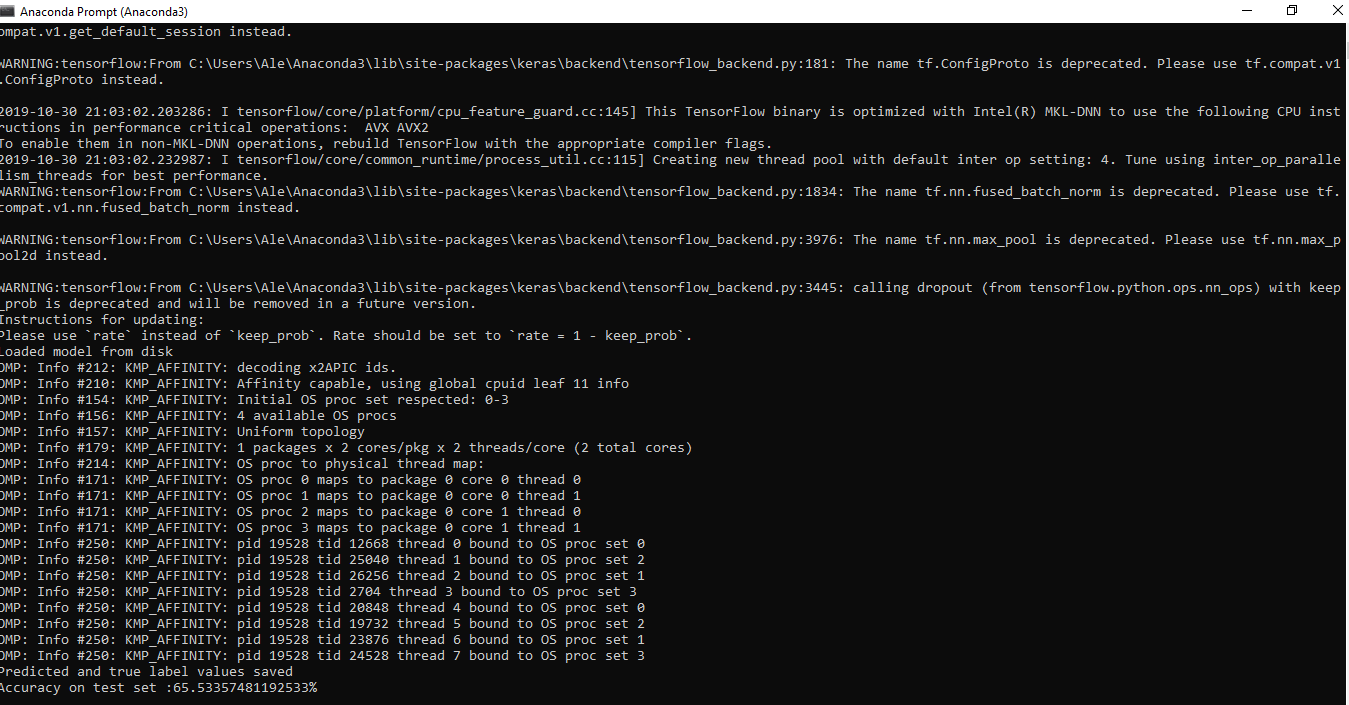
\includegraphics{accuracy-test-program.png}
% 	\caption{Accuracy Results}
% 	\label{swarmsize}
% \end{figure}

\begin{itemize}
  \item FER: Traning acc (90\% from dataset): 98.64\% - Test acc (10\% from dataset): 67.24\% (a bit of overfitting)
  \item CAFFE: Traning acc (90\% from dataset): 89.94\% - Test acc (10\% from dataset): 67.59\% (a bit of overfitting) - also removing the open mouth images
\end{itemize}

\section{Discussion}
\label{section:discussion}

\begin{itemize}
	\item Is your hypothesis supported?
  \paragraph{}
  Yes
	\item What conclusions do the results support about the strengths and weaknesses of your method compared to other methods?
  \paragraph{}
  A more larger balanced dataset with kids faces is needed to obtain better results.
	\item How can the results be explained in terms of the underlying properties of the algorithm and/or the data.
  \paragraph{}
  Overfitting could happen sometimes (depends on the dataset), but the algorithm
  is pretty accurate as a human can be.
\end{itemize}

\bibliographystyle{plain}
%\bibliography{BibAll}
\begin{thebibliography}{1}
  \bibitem{stanford} http://deeplearning.stanford.edu/tutorial/supervised/ConvolutionalNeuralNetwork/

  \bibitem{machinelearning} https://machinelearningmastery.com/convolutional-layers-for-deep-learning-neural-networks/
  
  \bibitem{searchwhat} https://searchenterpriseai.techtarget.com/definition/convolutional-neural-network
  
  \bibitem{skymind} https://skymind.ai/wiki/convolutional-network
  
  \bibitem{skymindneural} https://skymind.ai/wiki/neural-network
  
  \bibitem{towards} https://towardsdatascience.com/a-comprehensive-guide-to-convolutional-neural-networks-the-eli5-way-3bd2b1164a53
  
\end{thebibliography}
\end{document}

